\documentclass[twoside]{AiTeX}



\title{PEV}
\author{A.L.K.}
\date{Diciembre 2021}
\begin{document}
%\datos{facultad}{universidad}{grado}{asignatura}{subtitulo}{autor}{curso}
\datos{Informática}{Universidad Complutense de Madrid}{Ingeniería informática}{Programación Evolutiva}{Memoria de la práctica 1}{Alejandro Barrachina Argudo \\ Adrià Carreras Bagur }{2023}
\portadaApuntes
\pagestyle{empty}
\tableofcontents
\pagestyle{empty}
\justify
\pagestyle{fancy}

\newpage

\chapterA{Capturas de funcionamiento}

\begin{figure}[H]
    \centering
    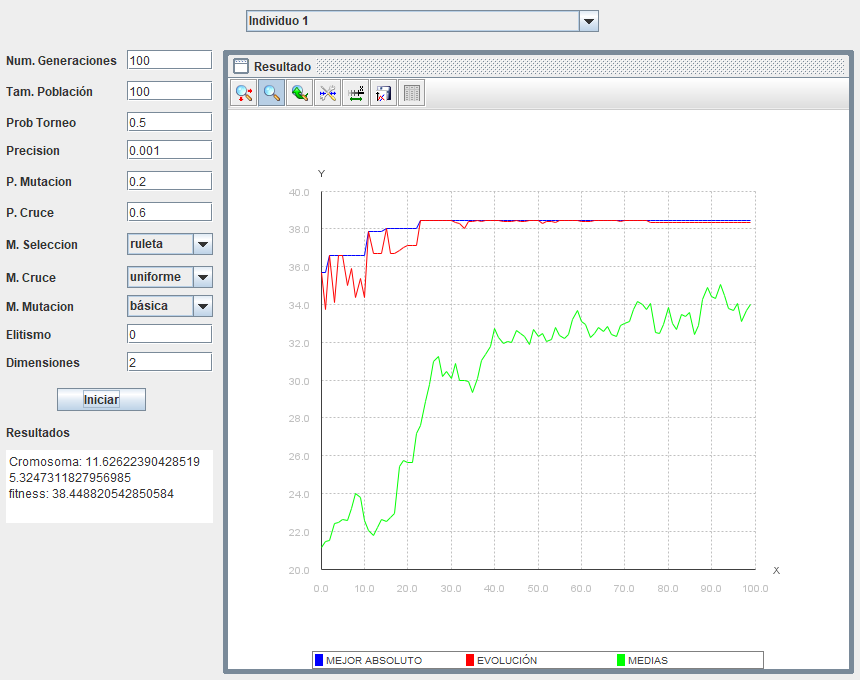
\includegraphics[width = \textwidth]{Images/Individuo1.png}
    \caption{Individuo 1}
\end{figure}

\begin{figure}[H]
    \centering
    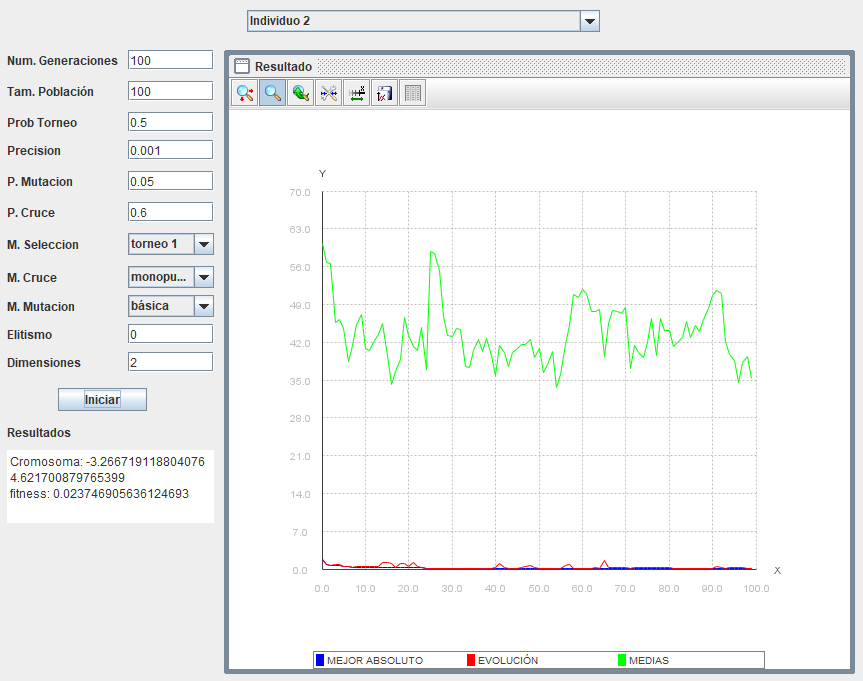
\includegraphics[width = \textwidth]{Images/Individuo2.png}
    \caption{Individuo 2}
\end{figure}

\begin{figure}[H]
    \centering
    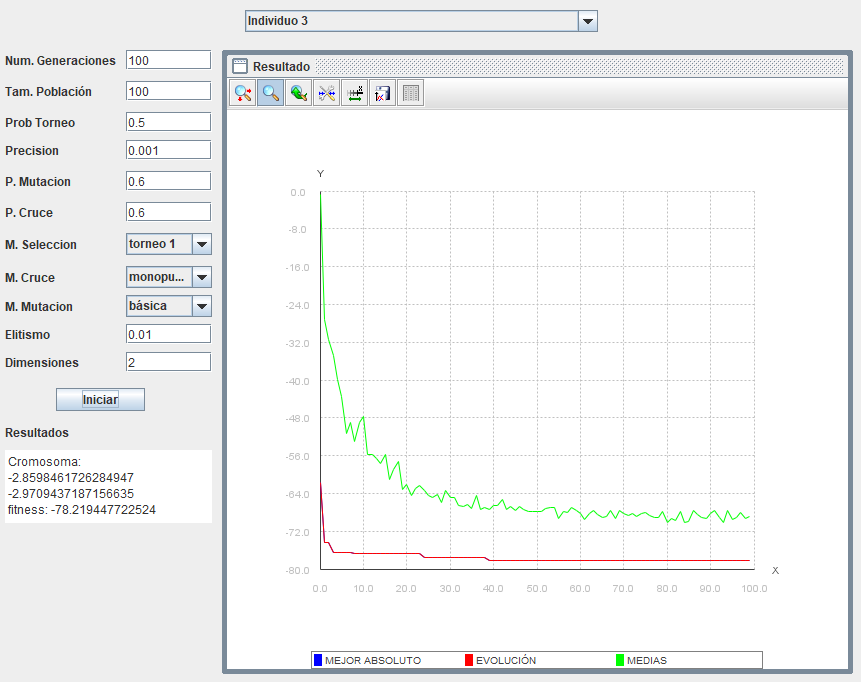
\includegraphics[width = \textwidth]{Images/Individuo3.png}
    \caption{Individuo 3}
\end{figure}

\begin{figure}[H]
    \centering
    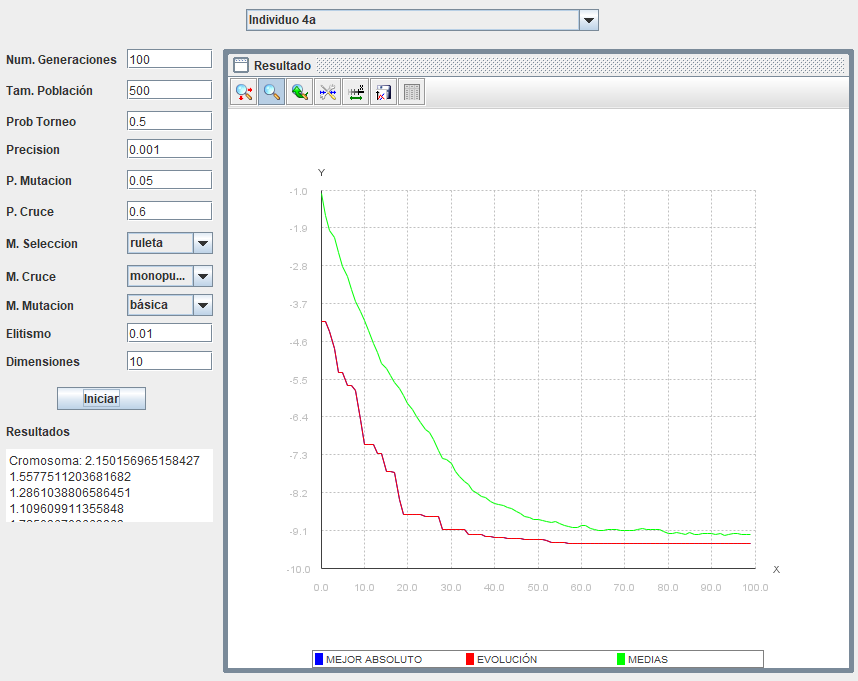
\includegraphics[width = \textwidth]{Images/Individuo4a.png}
    \caption{Individuo 4A}
\end{figure}

\begin{figure}[H]
    \centering
    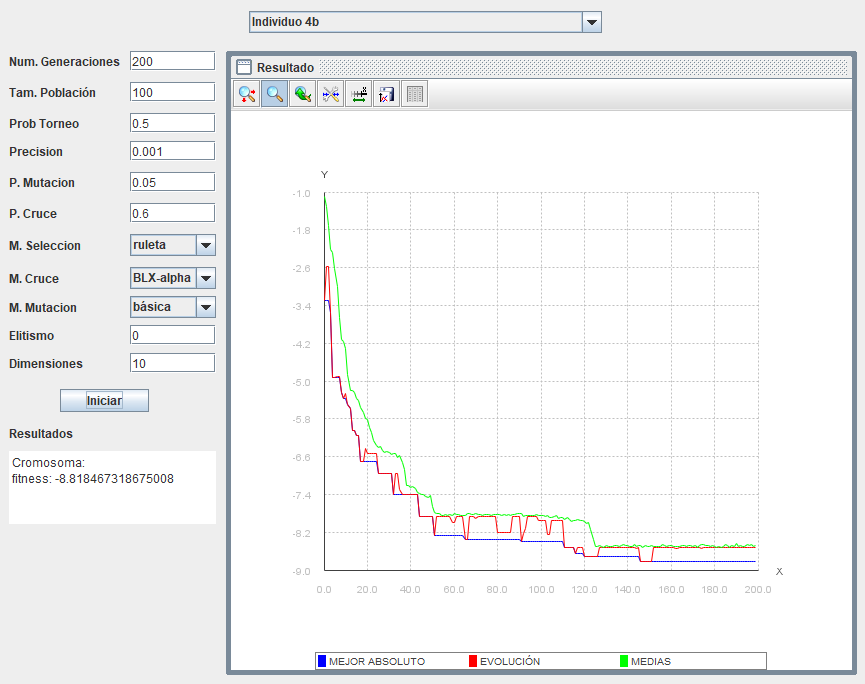
\includegraphics[width = \textwidth]{Images/Individuo4b.png}
    \caption{Individuo 4b}
\end{figure}

\chapterA{Ejecución y compilación de la práctica}

Al ser un proyecto en maven se puede importar directamente desde eclipse con la opción de abrir proyectos del sistema de archivos.

Para compilar el proyecto solo hay que darle al botón de \textit{run} y debería instalar las dependencias necesarias. Si no fuera así se puede ejecutar el comando \textit{mvn install} para instalar todas las dependencias.

Así mismo, el proyecto se puede correr desde el propio eclipse usando el botón de \textit{run}, usando la configuración de \textit{aplicación java} y como clase principal g02.Ventana.ventana.

El archivo jar se encuentra en la carpeta P01/target/


\chapterA{Distribución de trabajo}

Adrià ha hecho toda la GUI, parte de los cruces y parte de los individuos. Alejandro ha hecho la selección, parte de los cruces y parte de los individuos. La clase AlgoritmoGenetico se ha hecho entre los dos integrantes.


\end{document}
